% !TeX root = ../main.tex

\chapter{基于区间算数的整数缺陷检测}

C语言是一种面向过程的通用程序设计语言,由于其具有处理低级存储器、产生更少量的机器码以及不需要任何运行环境便可运行的特点,因而适用于操作系统等底层软件和需要高效运行的应用软件的编写。但也因为C语言的内存资源完全交由用户管理与控制,如果在程序设计与编写过程中考虑不全面或粗心大意,将会产生安全隐患。

其中,相当一部分的缺陷是由非法或错误的整型计算造成的:如整型溢出、除零异常、内存泄漏、缓冲区溢出等。在实际应用中,静态分析技术凭借其无需运行程序且分析路径的覆盖率高的特点,广泛应用于大规模软件的缺陷检测。通常,程序分析的精度与效率是不可兼得的:分析精度的提高往往伴随着效率的下降。平衡静态分析的精度与资源消耗,在不占用太多的资源下获得较好的分析精度一直是静态分析领域所重点关注的问题之一。

本章提出基于区间算数的整数缺陷检测技术,借助组合静态分析框架,在程序局部进行高精度的区间分析,对整体使用高效率的算法对各个局部分析结果进行组合,从而实现高效的C语言整数缺陷检测。本章的工作对提升现有工具的整数缺陷分析的精度和效率具有重要意义。

\section{引言}

若要判定程序中整型变量所参与的计算是否可能产生整型溢出、除零异常及缓冲区溢出等缺陷,传统的解决方案是使用抽象解释将程序中的整型变量上近似抽象为1个整数区间。结合数据流分析,得到整型变量在整数区间抽象域上的近似值,并以此判定整型变量的操作是否安全。

尽管该方法能够在简单逻辑代码上得到较好的分析效果,但由于抽象域的表示能力有限,在程序的逻辑分支复杂的情况下,因状态合并操作所带来的精度损失较大,通常经过数次操作即到达抽象域的上界。

\begin{figure}[htb]
	\begin{subfigure}[b]{.5\linewidth}
			\begin{lstlisting}[xleftmargin=.15\textwidth]
void funcA(int i) {
	int x;
	if (i > 0) {
		x = funcB(i) - 5;
	} else {
		x = 5 - funcB(i);
	}
	assert(x != 0);
}
			\end{lstlisting}
%			\caption{A listing}
	\end{subfigure}
	\begin{subfigure}[b]{.5\linewidth}
			\begin{lstlisting}[xleftmargin=.25\textwidth]
int funcB(int i) {
	int x;
	if (x > 3) {
		x = 3 - i;
	} else {
		x = i;
	}
	return x;
}
			\end{lstlisting}
%		   (-∞, 3]
%			\caption{A listing}
\end{subfigure}
	\caption{基于区间算数的缺陷检测方法举例}
	\label{fig:codeExampleForSignRange}
\end{figure}{\tiny }

考虑图\ref{fig:codeExampleForSignRange}所示代码:函数A作为程序的入口,通过用户输入得到整型数值i,并根据i的大小使用不同的逻辑调用函数B并处理函数返回值。这里为讨论方便起见,规定int可表示所有整数值。若使用传统的基于整数区间抽象的数据流分析算法进行程序分析,易知函数B的返回值范围是$ [-\infty, 3] $,则函数A中第4行x的取值范围是$ [-\infty, -2] $,第6行x的取值范围是$ [2, +\infty] $。在第8行,由于状态合并,x的取值范围是$ [-\infty, +\infty] $,这将导致目标属性不成立。但实际上x的取值范围不包含0,目标属性是安全的。

为了解决上述问题,进一步提高程序分析的精度,本章提出了基于区间算数的整数缺陷检测技术,并在基于CPAchecker\cite{beyer2007configurable}的可配置的组合静态分析工具Tsmart上进行了实现。经过实验,XXX。

\section{预备知识}

%\subsection{静态分析}
%
%静态分析是指在不运行代码的情况下,对程序源代码进行行为分析,从而判定程序是否满足某种特性。在代码的审查与优化、代码的缺陷分析与修复等方面有着大量应用。衡量静态分析技术的优劣通常考虑两个方面:分析精度和分析效率。分析精度用于衡量程序的实际行为与分析结果之间的匹配程度,分析效率则注重程序分析所消耗的资源大小,包括时间、存储的开销等。通常,程序分析的精度与效率是不可兼得的:分析精度的提高往往伴随着分析效率的下降,在实际应用中,我们往往需要平衡静态分析的精度与资源消耗,在不占用太多的资源下获得较好的分析精度一直是静态分析领域所重点关注的问题之一。

\subsection{控制流自动机}

控制流自动机(Control-flow Automaton,CFA)是命令式程序的一种语义等价表示方法,它是一个有向图:
\begin{definition}
	CFA可表示为有向图$ G = (N, E) $:$ N $是节点的集合,节点$ n \in N $表示程序的状态。$ E \subseteq N \times Ops \times N $是边的集合,有向边$ e = (n, op, n') \in E $表示从某个程序状态到下一个程序状态的过程,其中,$ Ops $是状态之间所执行的指令。一般地,我们用$ pred(e) $表示边$ e $的前驱节点$ n $,用$ succ(e) $表示边$ e $的后继节点$ n' $,用$ act(e) $表示边$ e $所执行的动作$ op $。
\end{definition}

在本文中,若无特殊说明,CFA是LLVM-IR语言上的等价表示,有向边$ e $根据其表示的指令的不同,可分为如下几类:
\begin{itemize}
	\item 空白边(BlankEdge):表示没有执行动作的边。$ act(e) = \varepsilon $;
	\item 假设边(AssumeEdge):描述了假设条件是否成立。$ act(e) = (\%cmp) $
\end{itemize}

\subsection{可配置程序分析框架} 

可配置程序分析(Configurable Program Analysis,CPA)是一种通用的程序分析框架,通过设计并配置相关参数,实现在同一框架下完成多种不同的静态分析任务。通常,CPA框架将程序源代码转化为语义等价的控制流自动机并在CFA上多次应用静态分析算法实现程序分析。其中,CFA是源程序的等价表示,可描述为有向图。其节点表示指令位置、边表示控制流操作,如变量声明、运算、赋值、函数调用等。在分析时,我们常将内存地址抽象为内存位置,如访问路径\cite{cheng2000modular}等。

CPA算法的一次分析可表示为四元组$ \mathbb{D} = (D, \rightsquigarrow, merge, stop) $。其中,$ D $为抽象域;$ \rightsquigarrow $为转移关系,规定了在不同的控制流操作下,给定的抽象状态如何转移到新的抽象状态;$ merge $为状态合并算子;$ stop $为状态覆盖算子。

算法\ref{alg:CPA算法}描述了CPA的算法流程:算法以分析$ \mathbb{D}$、CFA图$ G $和初始状态$ e_0 \in E $作为输入,通过维护工作队列$ waitlist $和可达状态集$ R $并根据转移关系$ \rightsquigarrow $来计算当前状态$ e $的后继状态。工作队列和可达集的维护算法如算法\ref{alg:UpdateRW}所示,对每个后继状态$ e' $使用$ merge $算子来更新所有可达状态,如果可达状态$ e'' $被更新,则将该状态加入到等待队列$ waitlist $中以更新其后继状态。如果更新后的可达状态无法覆盖$ e' $,则将该状态分别加入$ waitlist $和可达集中。

\begin{algorithm}[H]
	\caption{CPA算法}
	\label{alg:CPA算法}
	\begin{algorithmic}[1]
		
		\Require $ \mathbb{D} = (D, \rightsquigarrow, merge, stop) $,CFA图$ G $,初始状态$ e_0 \in E $
		\Ensure 可达状态集$ R $
		
		\State $ waitlist \gets \left\{ e_0 \right\} , R \gets \left\{ e_0 \right\}$
		\While{$ waitlist \ne \emptyset $}
			\State 取出$ waitlist $的首元素$ e $;
			\ForAll{$ e' $满足$ e \rightsquigarrow e' $}
				\State \Call{UpdateRW}{$ e', R, waitlist, merge, stop $};
			\EndFor
		\EndWhile
		
	\end{algorithmic}
\end{algorithm}

\begin{algorithm}[H]
	\caption{UpdateRW算法}
	\label{alg:UpdateRW}
	\begin{algorithmic}[1]
		
		\Function{UpdateRW}{$ e', R, waitlist, merge, stop $}
			\ForAll{$ e' \in R $}
				\State $ e_{new}  \gets merge(e, e')$;
				\If{$ e_{new} \ne e' $}
					\State $ waitlist \gets (waitlist \cup \{e_{new}\}) \setminus \{e'\} $;
					\State $ R \gets (R \cup \{e_{new}\}) \setminus \{e'\} $;
				\EndIf
			\EndFor
			\If{$\neg stop(e, R)$}
				\State $ waitlist \gets (waitlist \cup \{e\}) $;
				\State $ R \gets R \cup \{e\} $;
			\EndIf
		\EndFunction
		
	\end{algorithmic}
\end{algorithm}

\section{基于线性空间的抽象域设计}

本节介绍基于线性空间的抽象域,抽象域的组成结构如图\ref{fig:Domains}所示。ApRangeState为程序变量在线性空间的抽象表示,它包含变量的访问路径、取值范围、符号等信息。

\begin{figure}[H]
	\centering
	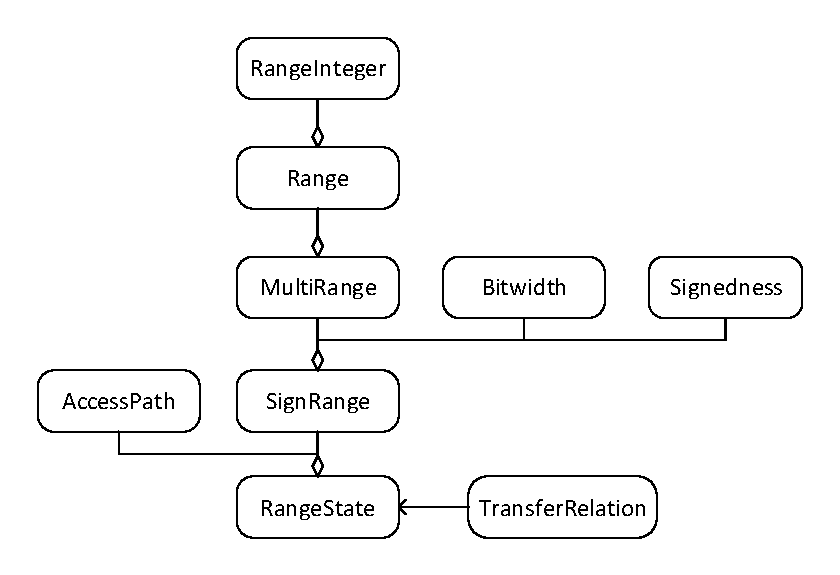
\includegraphics{Domains.pdf}
	\caption{抽象域的组成}
	\label{fig:Domains}
\end{figure}

\subsection{扩展的整数(RangeInteger)理论域}

整型变量的可能取值是一个整数的集合,在这里我们使用扩展的整数RangeInteger来表示一个具体的整数,它是整数域$ \mathbf{Z} $的一个拓展。

记$ \mathbf{I} := \mathbf{Z} \cup \{ +\infty, -\infty \}  $为扩展的整数理论域。其偏序关系($ \le $)为$ \mathbf{Z} $上的自然扩展,对于元素$ -\infty $与$ +\infty $,规定$ -\infty < +\infty $,且对任意$ x \in \mathbf{Z} $,有$ x < +\infty $以及$ -\infty < x $。特殊地,$ -\infty $与$ -\infty $、$ +\infty $与$ +\infty $无法比较。

对于元素$ -\infty $或$ +\infty $参与的运算,其规则如表\ref{tab:Integer运算规则}所示。其中,函数$ signum $为取符号数,具体定义如下:
\begin{align}
	signum(x) := \begin{cases}
		1 & (x \in \mathbf{Z} \land x > 0) \lor x = +\infty\\
		0 & x = 0\\
		-1 & (x \in \mathbf{Z} \land x < 0) \lor x = -\infty
	\end{cases}
\end{align}

特别的,元素$ +\infty $与$ -\infty $所参与的某些运算是未定义的。这样的运算在表中记录为undef,如$ (+\infty) +_I (-\infty), (+\infty) \div_I (+\infty)  $等。

\begin{table}[H]
	\centering
	\begin{minipage}[t]{0.85\linewidth} 
		\caption[RangeInteger运算规则]{RangeInteger运算规则}
		\label{tab:Integer运算规则}
		\begin{tabularx}{\linewidth}{cclc}
			\toprule[1.5pt]
			{\heiti 运算} & {\heiti 符号} & \multicolumn{1}{c}{\heiti 运算规则} \\\midrule[1pt]
			
			negate & $ neg_I $ & $  neg_I(x) :=  \begin{cases}
				-x & x \ne \pm\infty\\
				-\infty & x = +\infty\\
				+\infty & x = -\infty\\
			\end{cases}$\\
			
			add &$  +_I $ & $ x +_I y :=  \begin{cases}
				x + y & x, y \ne \pm\infty\\
				x & x = \pm\infty \land y \ne \pm\infty\\
				y & x \ne \pm\infty \land y = \pm\infty\\
				x & x, y = \pm\infty \land signum(x) = signum(y) \\
				\text{undef} & \text{other cases}
			\end{cases}$ \\
			
			subtract & $ -_I $ & $ x -_I y := \begin{cases}
				x - y & x, y \ne \pm\infty\\
				x & x = \pm\infty \land y \ne \pm\infty\\
				neg(y) & x \ne \pm\infty \land y = \pm\infty\\
				x & x, y = \pm\infty \land signum(x) \ne signum(y) \\
				\text{undef} & \text{other cases}
			\end{cases} $\\
			
			multiply & $ \times_I $ & $ x \times_I y := \begin{cases}
				x \times y & x, y \ne \pm\infty\\
				+\infty & signum(x) \times signum(y) > 0\\
				-\infty & signum(x) \times signum(y) < 0\\
				\text{undef} & \text{other cases}
			\end{cases} $\\
			
			\begin{tabular}{c}
				divide\\
				$ (y \ne 0) $\\
			\end{tabular} & $ \div_I $ & $ x \div_I y := \begin{cases}
				x \div y & x, y \ne \pm\infty\\
				0 & x \ne \pm\infty \land y = \pm\infty\\
				+\infty \times_I signum(x \times_I y) & x = \pm\infty \land y \ne \pm\infty\\				
				\text{undef} & \text{other cases}
			\end{cases} $\\
			
			\begin{tabular}{c}
				modular\\
				$ (y > 0) $\\
			\end{tabular} & $ mod_I $ & $ x \mod_I y := \begin{cases}
			x \mod y & x, y \ne \pm\infty\\
			x & x \ge 0 \land y = +\infty\\
			y & x < 0 \land y =+\infty\\
			\text{undef} & \text{other cases}
			\end{cases} $\\
			
			\begin{tabular}{c}
				and\\
				or\\
				xor\\
				shl\\
				shr
			\end{tabular} & \begin{tabular}{c}
			$ and_I $\\
			$ or_I $\\
			$ xor_I $\\
			$ <<_I $\\
			$ >>_I $
		\end{tabular} & $ x \cdot_{op_I} y := \begin{cases}
			x \cdot_{op} y & x, y \ne \pm\infty\\
			\text{undef} & \text{other cases}
			\end{cases} $\\
		\bottomrule[1.5pt]
		\end{tabularx}
		\end{minipage}
\end{table}


\subsection{线性区间理论域Range}

线性区间理论域Range一个整数区间,表示整型变量的可能取值范围,是由两个整数$ x, y $构成的二元组。这里,$ x, y $为扩展的整数域RangeInteger上的元素,其定义与偏序关系定义如下。

\begin{definition}
	线性区间理论域$ D_R :=  \{ [x, y] | x \in \mathbf{I}, y \in \mathbf{I}, x \le y \} \cup \{ \emptyset \}$是一个半格:	
	\begin{itemize}
		\item $ D_R $上的最大元($ \top_R $)是$ [-\infty, +\infty] $,最小元($ \bot_R $)是空集$ \emptyset $;
		\item $ D_R $上的偏序关系($ \le_R $)定义为:\\	
		\centerline{$ [x_1, y_1] \le_R [x_2, y_2] \iff x_2 \le x_1 \land y_1 \le y_2 $;}
		\item $ D_R $上的上确界操作($ \sqcup_R $)定义为:\\	
		\centerline{$ [x_1, y_1] \sqcup_R [x_2, y_2] := [\min(x_1, x_2), \max(y_1, y_2)] $,}  \\
		此处$ \max $和$ \min $为在$ \mathbf{I} $上的自然扩展。
	\end{itemize}
\end{definition}

我们在Range上定义一些基础的运算操作,其运算规则如表\ref{tab:Range运算规则}所示。值得注意的是,最小元$ \bot_R $与任何元素的计算结果均为$ \bot_R $,为表示方便,在表中默认操作数均不为$ \bot_R $。

\begin{longtable}{cclc}
	\caption[Range运算规则]{Range运算规则}
	\label{tab:Range运算规则}  \\ % add \\ command to tell LaTeX to start a new line	
	
	% Appear table header at the first page as well
	\toprule[1.5pt]	
	{\heiti 运算} & {\heiti 符号} & \multicolumn{1}{c}{\heiti 运算规则} \\
	\midrule[1pt]
	\endfirsthead
	
	% Appear the table header at the top of every page
	\multicolumn{3}{c}{续表~\thetable\hskip1em Range运算规则}\\
	\toprule[1.5pt]	
	{\heiti 运算} & {\heiti 符号} & \multicolumn{1}{c}{\heiti 运算规则} \\
	\midrule[1pt]
	\endhead 
	
	% Appear \hline at the bottom of every page
	\hline
	\multicolumn{3}{r}{续下页}
	\endfoot 
	\endlastfoot
	
	% data begins here	
	negate & $ neg_R $ & $  neg_R([x, y]) := [[neg_I(x), neg_I(y)]]_R$\\
	
	add & $ +_R $ & $ [x_1, y_1] +_R [x_2, y_2] := [[x_1 +_I x_2, y_1 +_I y_2]]_R $\\
	
	subtract & $ -_R $ & $ [x_1, y_1] -_R [x_2, y_2] :=  [[	x_1 -_I y_2, y_1 -_I x_2]]_R$\\
	
	multiply & $ \times_R $ & \begin{tabular}{lc}
		$ [x_1, y_1] \times_R [x_2, y_2] := $\\
		$ [\min(vals), \max(vals)], vals = \{x_1, y_1\} \times_{\times_I} \{x_2, y_2\} $
	\end{tabular}\\

	\begin{tabular}{c}				
		divide\\
		$ (op_2 \ne 0)$
	\end{tabular}& $ \div_R $ & \begin{tabular}{lc}
		$  [x_1, y_1] \div_R [x_2, y_2] := $ \\
		$ \begin{cases}
			[\min(vals), \max(vals)] &\begin{tabular}{lc}
				$ 0 \notin [x_2, y_2]$,  \\
				$ vals = \{x_1, y_1\} \times_{\div_I} \{x_2, y_2\}  $
			\end{tabular}\\
			[x_1, y_1] \div_R [1, y_2] & x_2 = 0\\
			[x_1, y_1] \div_R [x_2, -1] & y_2 = 0\\
			[neg(upper), upper] & \begin{tabular}{lc}
				$ x_2 < 0 < y_2,  $ \\
				$ upper = \max(|x_1|, |y_1|) $
			\end{tabular}\\
		\end{cases} $
	\end{tabular}\\

	\begin{tabular}{c}
		modular\\
		$ (op_2 \ne 0) $\\
	\end{tabular} & $ mod_R $ & \begin{tabular}{lc}
		$ [x_1, y_1] \mod_R [x_2, y_2] := $ \\
		$ \begin{cases}
			op_1 -_R op_2 \times_R times_1 & \begin{tabular}{lc}
				$ x_2 > 0 $\\
				$ times_1 = op_1 \div_R op_2 +_R [1, 1] $
			\end{tabular}\\
			
			op_1 -_R op_2 \times_R times_2 & \begin{tabular}{lc}
			$ y_2 < 0 $\\
			$ times_2 = op_1 \div_R op_2 -_R [1, 1] $
			\end{tabular}\\
		\end{cases} $
	\end{tabular}\\

	\begin{tabular}{c}
		and\\
	\end{tabular} & $ and_R $ & \begin{tabular}{lc}
		$ [x_1, y_1]\  and_R \ [x_2, y_2] := $ \\
		$ \begin{cases}
			x_1 \ and_I \ y_1 & x_1 = y_1 \land x_2 = y_2\\
			[0, y_1] & x_1 = y_1 \ge 0\\
			[0, y_2] & x_2 = y_2 \ge 0\\
			[0, +\infty] & x_1 \ge 0 \lor x_2 \ge 0\\
			[-\infty, -1] & y_1 < 0 \land y_2 < 0\\
			[-\infty, +\infty] & \text{other cases}
		\end{cases} $
	\end{tabular}\\
	
	\begin{tabular}{c}
		or\\
	\end{tabular} & $ or_R $ & \begin{tabular}{lc}
		$ [x_1, y_1] \ or_R \  [x_2, y_2] := $ \\
		$ \begin{cases}
			x_1 \ or_I \  y_1 & x_1 = y_1 \land x_2 = y_2\\
			[-1, -1] & x_1 = y_1 = -1 \lor x_2 = y_2 = -1\\
			[\max(x_1, x_2), +\infty] & x_1 \ge 0 \land x_2 \ge 0\\
			[-\infty, -1] & y_1 < 0 \lor y_2 < 0\\
			[-\infty, +\infty] & \text{other cases}
		\end{cases} $
	\end{tabular}\\

	\begin{tabular}{c}
		xor\\
	\end{tabular} & $ xor_R $ & \begin{tabular}{lc}
		$ [x_1, y_1] \ xor_R \  [x_2, y_2] := $ \\
		$ \begin{cases}
			x_1 \ xor_I \  y_1 & x_1 = y_1 \land x_2 = y_2\\
			[x_1, y_1] & x_2 = y_2 = 0\\
			[x_2, y_2] & x_1 = y_1 = 0\\
			[-\infty, +\infty] & x_1 \times_I x_2 < 0 \lor x_2 \times_I x_2 < 0\\
			[0, +\infty] & (x_1 \ge 0 \land x_2 \ge 0) \lor (y_1 < 0 \land y_2 < 0)\\
			[-\infty, -1] & \text{other cases}
		\end{cases} $
	\end{tabular}\\

	\begin{tabular}{c}
		shl\\
	\end{tabular} & $ <<_R $ & \begin{tabular}{lc}
		$ [x_1, y_1] <<_R  [x_2, y_2] := $ \\
		$ \begin{cases}
			\emptyset & y_2 < 0\\
			[x_1, y_1] <<_R [0, y_2] & 0 \in [x_2, y_2]\\
			[\min(vals), \max(vals)] & \text{other cases}, vals = \{x_1, y_1\} \times_{<<_I} \{x_2, y_2\}
		\end{cases} $
	\end{tabular}\\

	\begin{tabular}{c}
		shr\\
	\end{tabular} & $ >>_R $ & \begin{tabular}{lc}
		$ [x_1, y_1] >>_R  [x_2, y_2] := $ \\
		$ \begin{cases}
		\emptyset & y_2 < 0\\
		[x_1, y_1] >>_R [0, y_2] & 0 \in [x_2, y_2]\\
		[\min(vals), \max(vals)] & \text{other cases}, vals = \{x_1, y_1\} \times_{>>_I} \{x_2, y_2\}
		\end{cases} $
	\end{tabular}\\
	% more data here
\bottomrule[1.5pt]
\end{longtable}

在表格中,我们定义了构造函数$ [[\cdot]]_R $,利用它可以方便的构造Range:
\begin{align}
[[x, y]]_R := \begin{cases}
[x, y] & (x, y \text{ is comparable}) \land x \le y\\
[y, x] & (x, y \text{ is comparable}) \land x > y\\
\emptyset & \text{other cases}
\end{cases}
\end{align}

同时,为了进一步简化书写,我们定义了集合上的操作$ \times_{\cdot_{op}} $。对集合$ setA $和$ setB $,有:
\begin{align}
setA  \times_{\cdot_{op}} setB =  \{ e_i \cdot_{op} e_j \, | \, e_i \in setA, e_j \in setB \} 
\end{align}

Range的比较规则定义如下:
\begin{align}
	[x_1, y_1] < [x_2, y_2] \iff y_1 < x_2\\
	[x_1, y_1] > [x_2, y_2] \iff x_1 > y_2
\end{align}

\subsection{线性多区间(MultiRange)理论域}

通过分析图\ref{fig:codeExampleForSignRange}所示的代码案例,易知在整型变量分析时,使用单独的线性区间Range会造成一定程度的精度损失,这时需要提供一个更为精确的理论域来对整型变量的取值范围做抽象。

本小节介绍线性多区间MultiRange,它是由0到$ L_{MR} $个Range构成的有序的区间列表,通过使用多个Range区间,MultiRange能够提供更贴近实际域的变量取值区间表示。当$ L_{MR}  \rightarrow \infty $时,MultiRange能够精确表示整型变量的每一个可能取值,其表示能力和RangeInteger相同;当$ L_{MR} = 1 $时,MultiRange退化为Range。

在实际应用中,由于MultiRange可以根据需要通过改变$ L_{MR} $值的大小灵活改变理论域的表示精度,从而可以十分灵活的针对不同情况,优化程序分析的分析效率与分析精度。

\begin{definition}
	线性多区间理论域$ D_{MR}  := \{ [range_1, \dots, range_n] \ | \ 0 \le n \le L_{MR},  $
	
	$range_1 < \dots < range_n, range_i \in D_R\}$是一个半格:
	\begin{itemize}
		\item $ D_{MR} $上的最大元($\, \top_{MR} $)是$ [\top_R] $,最小元(\, $ \bot_{MR} $ ) 是$ [\,] $;
		
		\item $ D_{MR} $上的偏序关系($ \le_{MR} $)定义为:\\
			\centerline{$[rangeA_1, \dots, rangeA_m] \le_{MR} [rangeB_1, \dots, rangeB_n] \iff$}
			\centerline{$ \forall \ rangeA_i, \ \exists\  rangeB_j \text{ that} \ rangeA_i \le_R rangeB_j .\  (0 \le i \le m, 0 \le j \le n)$;}
			
		\item $ D_{MR} $上的上确界操作($ \sqcup_{MR} $)定义为:\\
			\centerline{$ [rangeA_1, \dots, rangeA_m] \sqcup_{MR} [rangeB_1, \dots, rangeB_n]  := $}
			\centerline{$ [[rangeA_1, \dots, rangeA_m, rangeB_1, \dots, rangeB_n]]_{MR} .\  (0 \le i \le m, 0 \le j \le n)$。}
	\end{itemize}
	
\end{definition}

上述的定义中使用了MultiRange的构造函数$ [[\cdot]]_{MR} $,其函数逻辑如算法\ref{alg:MultiRange}所示。该函数接受一个由Range组成的集合$ ranges $或直接给出待组合的Range列表$ range_1, range_2, \dots, range_n $。首先根据每个区间的左值和右值进行排序,得到有序的Range列表$ ranges $。并将$ ranges $中所有相互包含或相邻的区间进行合并,得到有序的且不互相包含、连接的区间列表$ nRanges $。为了保证得到的MultiRange中Range的个数小于$ L_{MR} $,在算法结束前不断合并前后相邻的且距离最小的Range直至其个数满足要求。

\begin{algorithm}[H]
	\caption{MultiRange的构造器$ [[\cdot]]_{MR} $}
	\label{alg:MultiRange}
	\begin{algorithmic}[1]
		
		\Require $ ranges = \{range_1, \dots, range_n\}, L_{MR} $
		\Ensure $ [nRange_1, \dots, nRange_m]. \ (0 \le m \le L_{MR})$
		
		\State sort $ ranges $ by $ range_{i}.x $ then by $ range_{i}.y $
		\State $ nRanges \gets \emptyset$
		\State $ [low, high] \gets$ peek$ (ranges) $
		\ForAll{$ range_i $ in $ ranges $}
			\If{$ range_i.x \le high +_I 1 $}
				\State $ high \gets \max(range_i.y, high) $
			\Else
				\State $ nRanges \gets nRanges \cup [low, high] $
				\State $ [low, high] \gets range_i $
			\EndIf
		\EndFor
		\While{$ size(nRanges) > L_{MR} $}
			\State pick range pair $ (nRange_i, nRange_{i+1} )$ in $ nRanges $ whose distance is shortest
			\State $ nRanges \gets (nRanges \setminus\{nRange_i, nRange_{i+1}\}) \cup (nRange_i \sqcup_R nRange_{i+1}) $
			\State sort $ nRanges $ by $ nRange_{i}.x $ then by $ nRange_{i}.y $
		\EndWhile
		\\\Return $ toList(nRanges) $
		
	\end{algorithmic}
\end{algorithm}

我们同样在MultiRange上定义一些基础运算操作,如表\ref{tab:MultiRange运算规则}所示。为方便起见,记$ ranges = [range_i, \dots, range_n] $为一个MultiRange,它是一个有序Range列表。列表$ ranges $沿用集合上的符号$ \times_{\cdot_{op}} $,即$ rangesA \times_{\cdot_{op}} rangesB = toList(set_{\cdot_{op}}) $,其中$ set_{\cdot_{op}} = \{rangeA_i \cdot_{op} rangeB_j \, | \, rangeA_i \in rangesA, rangesB_j \in rangesB\, , 0 \le i \le m, 0 \le j \le n\}$。

\begin{longtable}[H]{cclc}
	\caption[MultiRange运算规则]{MultiRange运算规则}
	\label{tab:MultiRange运算规则}  \\ % add \\ command to tell LaTeX to start a new line	
	
	% Appear table header at the first page as well
	\toprule[1.5pt]	
	{\heiti 运算} & {\heiti 符号} & \multicolumn{1}{c}{\heiti 运算规则} \\
	\midrule[1pt]
	\endfirsthead
	
	% Appear the table header at the top of every page
	\multicolumn{3}{c}{续表~\thetable\hskip1em MultiRange运算规则}\\
	\toprule[1.5pt]	
	{\heiti 运算} & {\heiti 符号} & \multicolumn{1}{c}{\heiti 运算规则} \\
	\midrule[1pt]
	\endhead 
	
	% Appear \hline at the bottom of every page
	\hline
	\multicolumn{3}{r}{续下页}
	\endfoot 
	\endlastfoot
	
	% data begins here	
	negate & $ neg_{MR} $ & $  neg_{MR}(ranges) :=[[neg_R(range_1), \dots, neg_R(range_n)]]_{MR}$\\
	
	add & $ +_{MR} $ & \begin{tabular}{lc}
		$ rangesA +_{MR} rangesB  :=  [[rangesA \times_{+_R} rangesB]]_{MR}$
	\end{tabular}\\
	
	subtract & $ -_{MR} $ & \begin{tabular}{lc}
		$ rangesA -_{MR} rangesB  :=  [[rangesA \times_{-_R} rangesB]]_{MR} $
	\end{tabular}\\
	
	multiply & $ \times_{MR} $ & \begin{tabular}{lc}
		$ rangesA \times_{MR} rangesB :=  [[rangesA \times_{\times_R} rangesB]]_{MR} $
	\end{tabular}\\
	
	\begin{tabular}{c}				
		divide\\
		$ (op_2 \ne 0)$
	\end{tabular}& $ \div_{MR} $ & \begin{tabular}{lc}
		$ rangesA \div_{MR} rangesB :=   [[rangesA \times_{\div_R} rangesB]]_{MR} $
	\end{tabular}\\
	
	\begin{tabular}{c}
		modular\\
		$ (op_2 \ne 0) $\\
	\end{tabular} & $ \mod_{MR} $ & \begin{tabular}{lc}
		$ rangesA \mod_{MR}  \,  rangesB :=   [[rangesA \times_{\mod_R} rangesB]]_{MR} $
	\end{tabular}\\
	
	\begin{tabular}{c}
		and\\
	\end{tabular} & $ and_{MR} $ & \begin{tabular}{lc}
		$ rangesA  \,  and_{MR} \,   rangesB :=  [[rangesA \times_{and_R} rangesB]]_{MR} $
	\end{tabular}\\
	
	\begin{tabular}{c}
		or\\
	\end{tabular} & $ or_{MR} $ & \begin{tabular}{lc}
		$ rangesA  \,  or_{MR}  \,  rangesB :=  [[rangesA \times_{or_R} rangesB]]_{MR} $
	\end{tabular}\\
	
	\begin{tabular}{c}
		xor\\
	\end{tabular} & $ xor_{MR} $ & \begin{tabular}{lc}
		$ rangesA  \,  xor_{MR} \,   rangesB :=  [[rangesA \times_{xor_R} rangesB]]_{MR} $
	\end{tabular}\\
	
	\begin{tabular}{c}
		shl\\
	\end{tabular} & $ <<_{MR} $ & \begin{tabular}{lc}
		$ rangesA <<_{MR} rangesB :=  [[rangesA \times_{<<_R} rangesB]]_{MR} $
	\end{tabular}\\
	
	\begin{tabular}{c}
		shr\\
	\end{tabular} & $ >>_{MR} $ & \begin{tabular}{lc}
		$ rangesA >>_{MR} rangesB :=  [[rangesA \times_{>>_R} rangesB]]_{MR} $
	\end{tabular}\\
	% more data here
	\bottomrule[1.5pt]
\end{longtable}

由于MultiRange是由Range组成的有序列表,通过观察表\ref{tab:MultiRange运算规则}易知,其计算规则是Range计算规则的简单拓展。考虑两个只含有单独区间的MultiRange:$ rangesA = [[1, 3]]$,$ rangesB = [[2, 3]] $。$ rangesA \times_{MR} rangesB $按照上述计算规则的计算结果为$ [[1, 3] \times_R [2, 3]]  = [[2, 9]] $,而实际上$ rangesA \times_{MR} rangesB $的取值不可能为$ 5, 7, 8 $,计算存在精度丢失。为了解决上述问题,在后续章节提出优化方案,可进一步提升MultiRange的计算精度。

MultiRange的比较规则定义如下:
\begin{align}
	[rangeA_1, \dots, rangeA_m] < [rangeB_1, \dots, rangeB_n] \iff rangeA_m < rangeB_1\\
	[rangeA_1, \dots, rangeA_m] > [rangeB_1, \dots, rangeB_n] \iff rangeA_1 > rangeB_m
\end{align}

为了后续便利,在SignRange上定义如下函数:
\begin{itemize}
	\item $ kill(Range)$用于删除SignRange的表示集合中参数Range对应的部分。例如:\\
	对于$ signRange = ([[0, 255]], 8, Unsigned) $,有$ signRange.kill([10, 100]) = ([[0, 9], [101, 255]], 8, Unsigned) $。
\end{itemize}

\subsection{位敏感的线性区间(SignRange)理论域}

在前面介绍的RangeInteger、Range与MultiRange抽象表示均未考虑整型变量在计算机上的存储格式,即对变量在计算机中所占用字节的大小是不敏感(Bitwidth Sensitive)的。当程序分析需要考虑变量的字节大小时,这类抽象表示往往不能提供整型变量实际所能表示的整数范围。

位敏感的线性区间SignRange = (MultiRange, Bitwidth, Signedness)是一个三元组。其中,MultiRange是上小节所述的线性多区间;Bitwidth表征了变量在计算机中所占用的位宽;Signedness表征了存储于计算机中整型变量在程序中是以有符号还是无符号的形式解析的。

\begin{definition}
	定义符号性(Signedness)理论域$ D_S := \{Signed, Unsigned, Unknown\} $是一个半格:
	\begin{itemize}
		\item $ D_S $上的最大元($ \top_S $)是$ Unsigned $,最小元($ \bot_S $)是$ Unknown $;
		\item $ D_S $上的偏序关系($ \le_S $)定义为:\\
			\centerline{$ Unknown \le_S Signed \le_S Unknown $}
		\item $ D_S $上的上确界操作($ \sqcup_S $)定义为:\\
			\centerline{$ signedness_1 \sqcup_S signedness_2 := \begin{cases}
				signedness_2 & signedness_1 \le_S signedness_2\\
				signedness_1 & signedness_2 \le_S signedness_1\\
				\end{cases} $}
	\end{itemize}
\end{definition}

引入符号性理论域意味着一个整形变量取值范围会随着符号性的不同而映射为不同的SignRange,尽管其在计算机内的存储内容是相同的(解释方式不同)。由于程序的这一特点,定义函数$ |_{to}(signedness) $用于转化同一整数取值范围的不同SignRange表示。方便起见,可将$ Signed, Unsigned, Unknown $分别记为$ S, U, N $。在此之前,先定义位敏感的线性区间SignRange的理论域:

\begin{definition}
	位敏感的线性区间理论域	$ D_{SR} := \{(ranges, bitwidth,  signedness) \, | \, $\\
	$ ranges \in D_{MR}, bitwidth \in \mathbf{Z^+}, signedness \in \{Signed, Unsigned, Unknown\}\} $是一个半格:
	\begin{itemize}
		\item $ D_{SR} $上的最大元($ \top_{SR} $)是$ (\top_{MR}, \top_{Z^+}, signedness) $,最小元($ \bot_{SR} $)是$ (\bot_{MR}, \bot_{\mathbf{Z}^+}, signedness)$;
		
		\item $ D_{SR} $上的偏序关系($ \le_{SR} $)定义为:\\
			\centerline{$ (rangesA, bitwidthA, signednessA) \le_{SR} (rangesB, bitwidthB, signednessB) \iff $}\\
			\centerline{$ (rangesA |_{to}(sgn(rangesB)) \le_{MR} rangesB) \land (bitwidthA \le bitwidthB) $;}
			
		\item $ D_{SR} $上的上确界操作($ \sqcup_{SR} $)定义为:\\
			\centerline{$ (rangesA, bitwidthA, signednessA) \sqcup_{SR} (rangesB, bitwidthB, signednessB)  := $}\\
			\centerline{$ (rangesA, bitwidth, signedness) , $}\\
			\centerline{其中,$ \begin{cases}
				signedness := \max(signednessA, signednessB)&\\
				bitwidth := \max(bitwidthA, bitwidthB)&\\
				ranges := rangesA |_{to}(signedness) \sqcup_{MR} rangesB |_{to}(signedness)&\\
				\end{cases}$。}
	\end{itemize}
\end{definition}

上述定义中,函数$ sgn::SignRange$为取SignRange的Signedness值。类似的,有$ width::SignRange $用于取SignRange的bitwidth值;$ range::SignRange $用于取SignRange的MultiRange值。


值得注意的是,$ getRanges(\top_{SR}) := \top_{MR} $。这意味着在SignRange中MultiRange的实际可取值范围比计算机表示范围大,这一特性将用于程序分析判定整形变量是否产生整形溢出。为了表示在计算机上固定位宽的整型变量的实际取值范围,定义函数$ top(SignRange) $和函数$ top(bitwidth, signedness) $用于计算在特定位宽下的整型变量以特定符号性解释的取值范围:

$ top(SignRange)  = top(bitwidth, signedness):=  $
\begin{align}
	\quad\quad\quad\begin{cases}
		[0, 2^{bitwidth} - 1]_{R} & signedness = Unsigned\\
		[-2^{bitwidth - 1}, 2^{bitwidth - 1} - 1]_{R} & signedness \in \{Signed, Unknown\}
	\end{cases}
\end{align}

函数$ |_{to} $的转换规则如算法\ref{alg:toUnsigned}和算法\ref{alg:toSigned}。

\begin{algorithm}[H]
	\caption{Convert2Unsigned, $ |_{to}(U) $}
	\label{alg:toUnsigned}
	\begin{algorithmic}[1]
		
		\Require $ signRange = (ranges, bitwidth, signedness) , signedness \in \{S, N\}$
		\Ensure new SignRange with Unsigned type
		
		\State $ convertVal \gets top(bitwidth, Unsigned).y + 1 $
		\State $ nRanges \gets \emptyset $
		\ForAll{$ range $ in $ range(signRange) $}
			\If{$ range < 0 $}
				\State $ nRanges \gets nRanges \cup (range +_R convertVal) $
			\ElsIf{$ range > -1 $}
				\State $ nRanges \gets nRanges \cup range $
			\Else
				\State $ nRanges \gets nRanges \cup ([range.x, -1] +_R convertVal) \cup [0, range.y] $
			\EndIf
		\EndFor
		\\\Return $ nSignRange = ([[nRanges]]_{MR}, bitwidth, Unsigned) $
	\end{algorithmic}
\end{algorithm}

\begin{algorithm}[H]
	\caption{Convert2Signed, $ |_{to}(S) $}
	\label{alg:toSigned}
	\begin{algorithmic}[1]
		
		\Require $ signRange = (ranges, bitwidth, signedness) , signedness \in \{U, N\}$
		\Ensure new SignRange with Signed type
		
		\State $ topVal \gets top(bitwidth, Signed) $
		\State $ convertVal \gets top(bitwidth, Unsigned).y + 1 $
		\State $ nRanges \gets \emptyset $
		\ForAll{$ range $ in $ range(signRange) $}
			\If{$ range < topVal + 1 $}
				\State $ nRanges \gets nRanges \cup range $
			\ElsIf{$ range > topVal $}
				\State $ nRanges \gets nRanges \cup (range -_R convertVal) $
			\Else
				\State $ nRanges \gets nRanges \cup [range.x, topVal] $
				\State $ nRanges \gets nRanges \cup ([topVal + 1, range.y] -_R convertVal) $
			\EndIf
		\EndFor
		\\\Return $ nSignRange = ([[nRanges]]_{MR}, bitwidth, Signed) $
	\end{algorithmic}
\end{algorithm}

与MultiRange相比,SignRange的计算规则着重考虑符号性。一般地,二元操作符在运算前需要统一其左右操作数的符号性。如无特殊说明,对操作数$ srA, srB $参与的二元运算$ srA \cdot_{op} srB $将按如下规则(Unifiy Signedness)更新自己的符号性并进行运算:

(1)当$ \cdot_{op} \in \{add, subtract, multiply, divide, mod\} $时,按下列规则更新符号性、位宽并运算:
\begin{align}{\label{align:Unify规则}}
	srA \cdot_{op} srB := \begin{cases}
		srA |_{to}(U) \cdot_{op} srB |_{to}(U) & sgn(srA) = U \lor sgn(srB) = U\\
		srA \cdot_{op} srB & sgn(srA) = N \land sgn(srB) = N\\
		srA |_{to}(S) \cdot_{op} srB |_{to}(S) & \text{other cases}
	\end{cases}\\
		width = width(srA) = width(srB) := \max(width(srA), width(srB)) 
\end{align}

(2)当$ \cdot_{op} \in \{and, or, xor\} $时,按下列规则运算,不更新位宽与符号性:
\begin{align}
	srA \cdot_{op} srB := srA |_{to}(S) \cdot_{op} srB |_{to}(S)
\end{align}

(3)当$ \cdot_{op} \in \{shl, shr\} $时,按下列规则更新符号性并运算,不更新位宽:
\begin{align}
	srA \cdot_{op} srB := srA \cdot_{op} srB |_{to}(U)
\end{align}

SignRange的计算规则如表\ref{tab:SignRange计算规则}所示。方便起见,记$ signRange = (ranges, width, signedness) $为一个SignRange。根据Unify Signedness规则,由于多数二元运算的操作数在运算前要更新符号性与位宽,因此表\ref{tab:SignRange计算规则}中若如无特殊说明,计算结果中的$ width, signedness $均为更新后的值。


\begin{longtable}{cclc}
	\caption[SignRange运算规则]{SignRange运算规则}
	\label{tab:SignRange计算规则}  \\ % add \\ command to tell LaTeX to start a new line	
	
	% Appear table header at the first page as well
	\toprule[1.5pt]	
	{\heiti 运算} & {\heiti 符号} & \multicolumn{1}{c}{\heiti 运算规则} \\
	\midrule[1pt]
	\endfirsthead
	
	% Appear the table header at the top of every page
	\multicolumn{3}{c}{续表~\thetable\hskip1em SignRange运算规则}\\
	\toprule[1.5pt]	
	{\heiti 运算} & {\heiti 符号} & \multicolumn{1}{c}{\heiti 运算规则} \\
	\midrule[1pt]
	\endhead 
	
	% Appear \hline at the bottom of every page
	\hline
	\multicolumn{3}{r}{续下页}
	\endfoot 
	\endlastfoot
	
	% data begins here	
	negate & $ neg_{SR} $ & \begin{tabular}{lc}
		$ neg_{SR}(signRange) :=  $\\
		$  \quad\begin{cases}
		(neg_{MR}(ranges), w, s) & s \in \{Signed, Unknown\}\\
		(neg_{MR}(ranges |_{to}(S)) |_{to}(U), w, s) & s = Unsigned
		\end{cases}$
		
	\end{tabular}\\
	
	add & $ +_{SR} $ & $ srA +_{SR} srB := (range(srA) +_{MR} range(srB), width, signedness) $\\
	
	subtract & $ -_{SR} $ & $ srA -_{SR} srB := (range(srA) -_{MR} range(srB), width, signedness) $\\
	
	multiply & $ \times_{SR} $ & $ srA \times_{SR} srB := (range(srA) \times_{MR} range(srB), width, signedness) $\\
	
	\begin{tabular}{c}				
		divide\\
		$ (op_2 \ne 0)$
	\end{tabular}& $ \div_{SR} $ & $ srA \div_{SR} srB := (range(srA) \div_{MR} range(srB), width, signedness) $\\
	
	\begin{tabular}{c}
		modular\\
		$ (op_2 \ne 0) $\\
	\end{tabular} & $ \mod_{SR} $ & \begin{tabular}{lc}
		$ srA \mod_{SR} \, srB := $\\
		$ \quad\quad\quad(range(srA) \mod_{MR} \, range(srB), width, signedness) $
	\end{tabular}\\
	
	\begin{tabular}{c}
		and\\
	\end{tabular} & $ and_{SR} $ & \begin{tabular}{lc}
		$ srA \, and_{SR} \, srB := $\\
		$ \quad\quad\quad(range(srA) \, and_{MR} \, range(srB), widthA, signednessA) $
	\end{tabular}\\
	
	\begin{tabular}{c}
		or\\
	\end{tabular} & $ or_{SR} $ & \begin{tabular}{lc}
		$ srA \, and_{SR} \, srB := $\\
		$ \quad\quad\quad(range(srA) \, and_{MR} \, range(srB), widthA, signednessA) $
	\end{tabular}\\
	
	\begin{tabular}{c}
		xor\\
	\end{tabular} & $ xor_{SR} $ & \begin{tabular}{lc}
		$ srA \, and_{SR} \, srB := $\\
		$ \quad\quad\quad(range(srA) \, and_{MR} \, range(srB), widthA, signednessA) $
	\end{tabular}\\
	
	\begin{tabular}{c}
		shl\\
	\end{tabular} & $ <<_{SR} $ & \begin{tabular}{lc}
		$ srA <<_{SR} srB := $\\
		$ \quad\quad\quad (range(srA) <<_{MR} range(srB'), widthA, signedness),  $\\
		$ \quad\quad\quad \text{in which } srB' := srB.kill([widthA, +\infty]).kill([-\infty, -1])$
	\end{tabular}\\
	
	\begin{tabular}{c}
		shr\\
	\end{tabular} & $ >>_{SR} $ & \begin{tabular}{lc}
		$ srA <<_{SR} srB := $\\
		$ \quad\quad\quad (range(srA) >>_{MR} range(srB'), widthA, signedness),  $\\
		$ \quad\quad\quad \text{in which } srB' := srB.kill([widthA, +\infty]).kill([-\infty, -1])$
	\end{tabular}\\
	% more data here
	\bottomrule[1.5pt]
\end{longtable}

在上一小节中,我们提到MultiRange在某些操作下会产生一定的精度丢失,这些精度丢失将会在后续章节进行修正。本节介绍的SignRange由于是MultiRange的扩展,其计算规则大部分调用了MultiRange的计算规则,因此对MultiRange的精度优化可以不加修改的继承到SignRange。

需要注意的是,由于SignRange是位敏感的,因此在进行shl和shr操作时,其计算精度仍可优化,优化方法将在后续章节随MultiRange的优化一同给出。

SignRange的比较规则定义如下:
\begin{align}
	srA < srB \iff range(srA') < range(srB')\\
	srA > srB \iff range(srA') > range(srB')
\end{align}

其中,$ srA', srB' $为根据Unify Signedness规则(\ref{align:Unify规则})更新符号性和位宽后得到的SignRange。

\subsection{\color{red}线性区间(ApRangeState)抽象域 $\rightarrow$求赐名}

通过上一小节的分析,使用位敏感的线性区间SignRange可以对整型变量的取值范围做精确的抽象表示和计算模拟,本节介绍的线性区间抽象域ApRangeState则是对控制流自动机(CFA)中所表示的程序状态的精确抽象,它描述了CFA上某程序状态下各个整型变量的取值范围。

线性区间抽象域ApRangeState = \{(AccessPath, SignRange)\}是一个由二元组(AccessPath, SignRange)组成的集合。它实际上是一个从AccessPath到SignRange的映射,描述了在某程序状态下,通过访问路径AccessPath访问得到的整型变量的表示范围SignRange。其中,AccessPath描述了一个整型变量在内存中的访问路径,通过这个访问路径,可以得到整型变量在内存中的唯一表示。

\begin{definition}
	线性区间抽象域$ D_{S_{AR}}  := \{ApRangeState \, | ApRangeState$ 是CFA上程序状态节点的抽象表示,$ ApRangeState =  \{(AccessPath, SignRange)\}   \}  $是一个{\color{red}半格?}
	\begin{itemize}
		\item $ D_{S_{AR}} $上的最大元($ \top_{S_{AR}} $)是,最小元($ \bot_{S_{AR}} $)是$ \{\emptyset\} $
		
		\item $ D_{S_{AR}} $上的偏序关系($ \le_{S_{AR}} $)定义为:\\
		\centerline{$ apRangeStateA \le_{S_{AR}} apRangeStateB \iff $}\\
		\centerline{$ apRangeStateA \subseteq apRangeStateB$ }
		
		\item $ D_{S_{AR}} $上的上确界操作($ \sqcup_{S_{AR}} $)定义为:\\
		\centerline{$ apRangeStateA \sqcup_{S_{AR}} apRangeStateB := $}\\
		\centerline{$ \{(ap, srA \sqcup_{SR} srB) | (ap, srA) \in apRangeStateA \lor (ap, srB) \in apRangeStateB\} $}
	\end{itemize}
\end{definition}

在CFA中,


线性区间抽象域上的变迁关系$ \rightsquigarrow_R $定义如下:

对于形如$ z = x \cdot_{op}  y$这样的操作边(Instruction Edge),其变迁关系为:

\begin{align}
\frac{X=\alpha_R(x), Y=\alpha_R(y)}{\alpha_R(Z) \leftarrow X \cdot_{op}Y} \quad\textsf{T-R-OP}
\end{align}

其中,$ \alpha_R $函数表示当前抽象状态中$ a $和$ b $的抽象表示(表示为$ D_R $中的区间)。这里,在区间上的运算操作是在$ I_R $和$ D_R $上运算的扩展,

\subsection{精度优化}

\section{基于区间算数的整数缺陷检测方法}

这里介绍checker的原理与检测规则、生成report的方法。

\section{模块实现}

介绍具体实现。

\section{实现方案} 

这里放工具图

\section{实验过程与结果}

这里介绍在Juliet与选取的几个项目上的测试结果。

\section{本章小结}

水。
assume, phi, instruction


















































